\section{文献回顾与研究假设}

\subsection{文献回顾}

\subsubsection{平台治理与算法监管}

数字平台治理研究经历了从技术视角向制度视角的范式转换。\citet{Kango2025}在《人本AI手册》中系统界定了算法治理的核心概念,强调算法不仅是技术工具,更是影响社会资源分配与权力结构的治理机制。早期研究聚焦于平台作为``双边市场''的经济属性\citep{Rochet2003, Armstrong2006},强调网络效应、定价策略与市场竞争。随着平台规模的扩大与社会影响的深化,学者开始关注平台的治理维度。\citet{Tiwana2010}提出平台生态系统理论,将平台视为由核心架构与互补者构成的共生系统,治理的核心在于协调多方利益、维护生态健康。\citet{Ghazawneh2013}进一步提出边界资源概念,分析平台如何通过API、规则与激励机制管理开发者行为。\citet{Parker2018}则从网络效应视角系统阐述了平台治理的独特逻辑,指出平台需要同时管理供给端(内容生产者)与需求端(用户),任何治理干预都可能产生跨边溢出效应。\citet{Jacobides2018}从生态系统视角分析了平台企业的治理逻辑与价值创造范式,\citet{Huber2013}进一步系统梳理了平台监管中契约治理与关系治理的互补与替代机制。焦豪\citeyearpar{JiaoHao2023}提出``数字平台生态观''这一理论新视角,强调数字经济时代企业需要建立与自身资源相匹配的数字平台,通过与利益相关者共同创造价值形成持续竞争优势。\citet{Degen2025}则从监管设计视角提出``平台治理标准类型''分类框架,主张针对不同类型平台实施差异化监管策略,为本文的分级分类治理分析提供了理论参照。

算法推荐系统的治理构成平台治理的新兴分支。算法作为平台的``隐性架构''\citep{Gillespie2014},通过个性化推荐深度介入用户的信息获取过程,成为事实上的``信息把关人''\citep{Gorwa2020}。\citet{Bucher2018}指出,算法权力体现在其``可供性''(affordance),算法不仅反映用户偏好,更主动塑造用户行为。这一视角在后续研究中得到进一步拓展,\citet{Gillespie2018}系统分析了平台作为``互联网守门人''的角色演变,强调算法已成为重构信息流通逻辑的核心力量;\citet{Katyal2019}则从法律视角分析了人工智能时代私人问责的边界问题。这一双向互动使得算法治理面临独特挑战:监管者既要约束算法的负面效应,又要避免过度干预导致系统效率损失\citep{Yeung2018}。

方法论层面,算法审计(algorithm audit)为理解算法行为提供了实证工具。\citet{Sandvig2014}系统梳理了算法审计的研究方法,提出了检测互联网平台歧视行为的实证框架;\citet{Diakopoulos2016}进一步将算法问责的理念应用于新闻推荐领域,发现算法推荐存在显著的议题设置效应。近年来,算法审计方法得到快速发展:\citet{Mousavi2024}以TikTok为对象审计了平台提供的算法解释功能,揭示了算法透明性承诺与实际操作之间的差距;\citet{Wang2024TwitterAudit}对比分析了Twitter/X算法推荐与时间线排序对新闻内容质量的差异化影响,发现算法推荐虽然降低了信息数量但提升了内容质量;\citet{Hosseinmardi2024}采用``反事实机器人''方法因果估计了YouTube推荐算法的效应,为算法审计的因果识别提供了方法论创新。国内学者亦对算法审计方法进行了本土化探索,师文和陈昌凤\citeyearpar{ShiWen2023}基于计算实验方法系统审计了国内主流平台算法的``主流化''偏向与``个性化''特质,为理解中国情境下的算法行为提供了实证基础。这些研究为本文的实证设计提供了方法论参考。

全球范围内,算法治理呈现差异化路径。欧盟采取``透明度+问责''模式,《通用数据保护条例》(GDPR)赋予用户``解释权'',《数字服务法》(DSA)要求平台披露推荐逻辑并接受第三方审计。\citet{Panigutti2025}系统梳理了DSA框架下算法风险调查的方法论路径,为平台合规与外部监督提供了操作指南。美国延续``自律为主''传统,但围绕《算法问责法案》的讨论日趋激烈\citep{Katyal2019}。李三希等\citeyearpar{LiSanxi2023}从产业组织视角考察了市场竞争对企业数据行为的影响,发现竞争能够有效约束企业过度收集消费者信息的动机,这为理解数据治理的市场化路径提供了理论基础。中国构建了全球最为系统的算法监管框架:2021年《互联网信息服务算法推荐管理规定》确立分级分类原则,2023年《生成式人工智能服务管理暂行办法》将监管延伸至大模型领域\citep{Creemers2022}。\citet{Xu2024}深入分析了中国算法监管的``打开黑箱''策略,指出中国监管模式强调``风险分级+事前审核''的制度组合;\citet{Sheehan2023}进一步揭示了中国AI监管的政策制定过程与多部门协调机制。\citet{Ulbricht2022}指出,算法监管已成为全球治理的成熟议题,各国在透明度、问责与风险分级等维度形成了差异化的制度路径。2024年``清朗行动''算法专项治理则以27项核验标准推动规则落地,体现了``风险分级+协同治理''的制度逻辑\citep{Gritsenko2022}。这一制度演进为本文提供了清晰的政策断点。

\subsubsection{注意力经济与信息分配}

注意力经济理论为理解平台内容生态提供了资源视角。\citet{Simon1996}最早指出,在信息过载时代,稀缺的不是信息本身而是处理信息的注意力。\citet{Davenport2001}将注意力定义为``对特定信息的聚焦心智参与'',强调其稀缺性、竞争性与货币化潜力。\citet{Webster2016}进一步提出``注意力市场''概念,将媒体竞争重新框定为对用户时间与心智份额的争夺。\citet{Wu2017}从历史视角系统梳理了注意力商业化的演进历程,揭示了数字时代注意力稀缺与算法分配的内在逻辑。\citet{OReilly2024}提出``算法注意力租金''概念,指出数字平台通过算法控制实现对用户注意力的系统性提取,形成独特的市场权力来源;\citet{Heitmayer2025}进一步发展了``注意力经济第二波''理论,将注意力概念化为社交媒体时代的``通用符号货币''。喻国明和刘彧晗\citeyearpar{YuGuoming2023}基于元传播视角提出,数字平台竞争已从``信息竞争''转向``认知竞争'',这一范式转型深刻重塑了注意力资源的获取与分配机制。

在数字平台情境下,注意力的分配呈现高度不均衡特征。\citet{Hindman2018}通过大规模网络流量分析揭示了``赢者通吃''格局,发现少数头部内容获取了不成比例的用户注意力,形成典型的幂律分布。\citet{Cui2023}以中国微博为研究对象,发现热门话题的注意力竞争呈现显著的``富者愈富''效应,平台干预能够有效调节这一格局。算法推荐系统可能加剧这一趋势:通过放大用户既有偏好,算法创造了``过滤气泡''(filter bubble)与``回音室''(echo chamber)效应\citep{Pariser2011, Sunstein2018}。然而,也有研究对此提出质疑。\citet{Guess2023}基于大规模实验发现,关闭算法推荐并未显著改善用户的信息多样性,暗示算法效应可能被高估。\citet{Hosanagar2014}的研究也表明,推荐系统对消费者信息多样性的影响存在高度异质性。\citet{Ahmmad2025}对过滤气泡与回音室研究进行了系统综述,指出算法对青年群体的影响存在显著异质性,过度简化的``信息茧房''叙事可能掩盖了更复杂的现实。喻国明和刘彧晗\citeyearpar{YuGuoming2024}进一步指出,``信息茧房''议题可能被过度渲染,个性化推荐并不必然导致用户视野收窄,算法推荐的实际效应需要更多实证检验。这一争论凸显了算法治理效果评估的重要性与复杂性。

注意力的零和特性对治理具有重要含义。\citet{Wu2017}指出,平台经济的核心商业模式是``注意力商人'',即通过免费内容吸引用户注意力,再将注意力出售给广告商。在此模式下,用户的总注意力构成平台收入的``天花板''。这意味着,对某一类型内容的监管干预可能引发注意力在不同类型间的再分配,本文将这一机制概念化为``水床效应''。

\subsubsection{内容质量与信息诱导}

内容质量劣化是算法治理的核心关切之一。信息差理论(information gap theory)为理解诱导性内容提供了心理学基础。\citet{Loewenstein1994}指出,当个体意识到知识缺口时会产生强烈好奇心,驱使其采取行动填补缺口。诱导性标题(clickbait)正是利用这一心理机制,通过制造标题与内容之间的语义悬念来操纵用户的注意力分配\citep{Golman2018}。\citet{Chakraborty2016}通过机器学习方法识别clickbait特征,发现疑问句式、悬念词汇、情感激发是典型策略。\citet{Chen2015}分析了clickbait的经济逻辑,指出在注意力竞争中,夸张标题能够获得更高点击率,但会损害用户信任与长期价值。

内容质量治理面临``逐底竞争''困境。\citet{Munger2020}指出,在算法驱动的信息环境中,内容生产者面临集体行动困境:个体理性(追求点击率)与集体理性(维护信息质量)相冲突,导致低质内容驱逐高质内容的``柠檬市场''效应。\citet{Berman2018}系统分析了算法策展对内容质量的影响,发现内容质量呈现分化趋势,专业媒体坚守内容标准,而用户生成内容更易陷入流量导向。\citet{Jhaver2019}基于Reddit的实证研究发现,内容审核透明性与用户信任之间存在显著正相关,这为治理干预提供了行为依据。平台治理的干预逻辑在于改变激励结构,使高质量内容获得更高回报\citep{Gillespie2018}。值得注意的是,内容审核可能产生非预期的溢出效应。\citet{Cima2025}采用双重差分方法研究大规模内容审核干预的异质性效应,发现审核行为在不同用户群体间产生差异化影响,部分群体甚至出现``反弹''现象;\citet{Gomes2024}则从公共健康视角分析了内容审核对数字减害实践的意外阻碍。这些发现提示,算法治理的效果评估需要关注监管的间接传导路径与非预期后果。然而,既有研究多聚焦于平台自治,对外部监管如何影响内容质量的实证分析相对匮乏。

\subsubsection{现有研究的不足与本文定位}

综上所述,现有文献在三个方面存在不足,构成本文的理论切入点。

第一,缺乏统一框架整合多维效应。平台治理文献分散于内容质量、信息多样性、用户行为等子领域,缺乏将多元治理效应纳入统一分析框架的理论尝试。尽管学者们在平台治理\citep{Parker2018, Tiwana2010}、算法权力\citep{Bucher2018, Katyal2019}等领域取得了重要进展,但鲜有研究将这些分散的理论视角系统整合。本文引入资源依赖理论,将用户注意力视为平台依赖的核心稀缺资源,从资源再配置视角统一解释内容质量分化、注意力去中心化、水床效应等多维效应。

第二,忽视监管的非预期后果。既有算法治理文献多聚焦于规范性讨论或单一目标评估\citep{Gritsenko2022, Ulbricht2022},缺乏对监管溢出效应的系统分析。本文提出``水床效应''概念,刻画在注意力零和约束下监管干预的间接传导路径,揭示质量提升与公共议题曝光度下降之间的潜在张力。

第三,因果识别研究稀缺。由于算法系统的``黑箱''特性和数据获取难题,既有研究多为描述性分析或规范性讨论。虽然\citet{Sandvig2014}和\citet{Diakopoulos2016}等学者发展了算法审计的方法论,但这些研究主要聚焦于算法行为的描述性刻画,而非政策干预的因果效应评估。本文利用2024年清朗行动提供的准自然实验场景,采用ITS与DID相结合的因果识别策略,提供算法治理效果的可信估计。

\subsection{理论框架与研究假设}

\subsubsection{资源依赖视角下的算法治理分析}

资源依赖理论(Resource Dependence Theory)认为,组织的生存与发展取决于其从外部环境获取关键资源的能力\citep{Pfeffer1978}。当组织高度依赖某一稀缺资源时,该资源的供给者将对组织行为产生深远影响。\citet{Yu2024PlatformDependence}系统梳理了平台依赖型创业的研究文献,指出平台生态系统中的资源依赖关系具有独特的双向性与动态性特征。本文将这一理论框架应用于数字平台情境,提出核心命题:用户注意力构成了数字平台最核心的稀缺资源,算法治理的本质是改变平台获取和配置注意力资源的成本结构与约束条件。

在数字平台生态系统中,注意力资源具有三个决定性特征\citep{OestreicherSinger2012, Berman2018}。第一,稀缺性:用户日均使用时长存在生理和时间约束,短期内缺乏弹性。第二,竞争性:注意力分配给某一话题必然减少其他话题的份额,形成典型的零和博弈格局。第三,不可再生性:注意力一旦消耗无法恢复。这三个特征共同构成了本文分析的基础约束——注意力总量守恒:各类内容获得的注意力之和等于平台可获取的总注意力预算。

基于资源依赖理论,算法治理通过两条路径影响平台行为:\textbf{成本路径}与\textbf{约束路径}。

\textbf{成本路径}:《算法专项治理清单指引》通过分级分类监管,对不同风险类别的内容施加差异化的合规要求,直接改变了平台的资源获取成本。监管后各类内容的成本变化取决于其风险等级和监管强度,且成本变化与风险等级正相关。由于社会类内容涉及公共利益、舆情风险等敏感领域,其风险等级显著高于娱乐类,导致社会类内容的合规成本大幅上升,而娱乐类成本基本稳定。这一差异化成本冲击将驱动平台对高风险内容实施更严格的质量筛选(对应假设H1),并在注意力总量守恒约束下引发跨类别的资源再分配(对应假设H3、H4)。

\textbf{约束路径}:监管同时施加了多样性约束,要求平台``不得利用算法操纵热点话题''、``保障信息内容多样性''。这直接改变了平台的可行域结构,限制了头部话题的注意力垄断能力(对应假设H2)。

面对差异化的成本冲击与新增约束,平台作为理性主体将重新优化其资源配置策略。平台的目标是在注意力总量守恒和多样性约束条件下最大化净收益。最优化条件要求各类内容的边际净收益相等。当社会类的合规成本上升时,平台需要减少社会类的注意力配置以提高其边际收益,并将释放的资源重新配置至成本较低的类别。在注意力总量守恒约束下,这一再配置过程产生了本文提出的``水床效应'':社会类注意力下降必然导致娱乐类和其他类别注意力上升。

基于上述理论框架,本文提出四项研究假设。这四项假设共同构成资源依赖视角下算法治理效应的完整图景:H1刻画成本路径的直接效应(质量筛选),H2刻画约束路径的直接效应(多样性提升),H3刻画资源总量约束下的再配置效应(水床效应),H4刻画再配置效应在微观层面的具体表现(密度分化)。

\subsubsection{假设H1:内容质量分化效应}

\textbf{理论逻辑}:资源依赖理论强调,组织会根据资源获取成本调整其行为策略\citep{Pfeffer1978}。分级分类监管的核心在于根据内容的舆论风险等级实施差异化监管强度。《算法专项治理清单指引》对涉及公共事件、舆情风险的社会类内容提出了更高的信息来源、事实核验和价值导向标准,而对娱乐类内容多采取``守住底线''的防御性姿态。

从资源依赖视角看,这一差异化监管直接转化为平台的差异化合规成本。社会类内容的合规成本大幅上升,包括强化内容审核成本、信息来源核查成本和违规问责风险成本;娱乐类内容的合规成本基本稳定。根据前述理论模型,当社会类合规成本上升时,平台的最优响应是提高社会类内容的质量门槛,通过``事前筛选''淘汰低质内容,从而降低单位内容的合规风险。换言之,社会类的质量门槛与其合规成本正相关,而娱乐类质量门槛基本不变。

在社会类内部,机构媒体相对自媒体将展现出更显著的质量提升。这源于两个机制:第一,源头筛选机制,平台在高风险领域优先选择机构媒体作为信息源头,因为机构媒体的内容规范性和可信度更高\citep{He2022},能够有效降低平台的合规风险;第二,信号显示机制,平台通过提升机构媒体占比向监管者传递合规信号,以获取监管合法性。

基于上述分析,提出假设H1:

\textbf{H1(内容质量分化)}:算法治理导致不同风险类别内容的质量呈现分化趋势,高风险内容质量显著提升,低风险内容质量基本稳定。

H1a:社会类话题的信息差指数(衡量标题信息诱导程度)在监管后显著下降

H1b:社会类内部,机构媒体相对自媒体的信息差净下降(DID估计量显著为负)

H1c:娱乐类话题的质量指标在监管前后无显著变化

\subsubsection{假设H2:注意力去中心化效应}

\textbf{理论逻辑}:资源依赖理论指出,外部约束的变化将迫使组织调整其资源配置模式\citep{Pfeffer1978}。《算法专项治理清单指引》明确要求平台``不得利用算法操纵热点话题''、``保障信息内容多样性''。这些监管条款构成了平台资源配置的硬约束边界,直接限制了头部话题的注意力垄断能力。

从资源配置视角看,多样性约束改变了平台的可行域结构。监管要求政策实施后话题分布的多样性水平(以Shannon熵衡量)必须高于政策实施前的最低标准,即监管提高了平台内容多样性的下限要求。该约束迫使平台压缩头部话题的资源配额、提升长尾话题的曝光机会。在注意力总量守恒的前提下,这意味着原本高度集中于少数话题的注意力将被重新分配至更广泛的话题集合。平台通过限制同一话题ID的上榜频次、设置话题轮换机制,从供给端切断了头部话题的垄断路径。

同时,监管还通过改变平台的风险收益函数,激励其主动提升内容多样性。单一话题过度曝光的违规概率在监管后显著上升,平台因话题过度集中而遭受监管处罚的预期成本相应增加。平台为规避监管风险而主动调低头部话题权重、提升长尾话题推荐权重。

基于上述分析,提出假设H2:

\textbf{H2(注意力去中心化)}:算法治理打破了热搜榜单的赢者通吃格局,注意力从少数头部话题向广泛的长尾话题再分配。

H2a:Shannon熵在监管后显著上升

H2b:HHI集中度指数在监管后显著下降

H2c:单条话题重复上榜次数和连续在榜时长在监管后显著下降

\subsubsection{假设H3:注意力再分配效应(水床效应)}

\textbf{理论逻辑}:水床效应是资源依赖理论在注意力总量守恒约束下的核心推论。资源依赖理论强调,当某一资源获取渠道受阻时,组织会转向替代性资源渠道\citep{Pfeffer1978}。在本文情境下,监管提高了社会类内容的获取成本,平台作为理性主体将调整其资源配置,将注意力从高成本领域转向低成本领域。

这一再分配过程同时受到供给侧和需求侧的双重驱动。从供给侧看,监管实施后社会类的``有效供给''因质量门槛提高和合规成本上升而下降。根据前述理论模型,平台选择的最优社会类内容数量与其合规成本呈负相关关系:当社会类合规成本上升时,平台倾向于减少社会类内容的供给数量。从需求侧看,用户的总注意力需求在短期内保持稳定,不会因监管而显著改变。在供需缺口下,用户将注意力转向替代性内容。由于娱乐类内容的审核成本相对较低,其成为承接溢出注意力的``蓄水池''。

这一``成本驱动''的再配置逻辑与用户行为的被动调整相互强化,共同塑造了``社会类紧缩与娱乐类扩张''的结构性格局。水床效应的存在可通过验证注意力总量守恒来间接证实:如果用户的总注意力预算在短期内保持稳定,则算法治理不应显著改变平台的总注意力供给量,而仅改变其在不同类型间的分配结构。具体表现为:平台总注意力保持基本稳定,但社会类注意力份额下降,娱乐类注意力份额相应上升。

基于上述分析,提出假设H3:

\textbf{H3(注意力再分配/水床效应)}:在注意力零和约束下,对社会类的监管强化将引发注意力向娱乐类的系统性转移。

H3a:社会类话题在热搜榜中的份额在监管后显著下降

H3b:娱乐类话题在热搜榜中的份额在监管后显著上升

H3c:周度总热度在监管前后无显著变化,验证注意力零和约束

\subsubsection{假设H4:注意力密度分化效应}

\textbf{理论逻辑}:注意力密度分化是水床效应在微观层面的具体表现,揭示了平台在宏观配额调整基础上的精细化响应策略。资源依赖理论指出,组织在资源约束下会采取差异化策略以最大化资源利用效率\citep{Pfeffer1978}。在本文情境下,社会类与娱乐类因其风险特征不同,将呈现截然不同的调整路径。

社会类预期呈现``少而精''的调整路径。根据前述分析,监管显著提高了社会类内容的准入门槛,低质内容在更严格的审核标准下被淘汰出局,导致上榜话题数量明显减少。与此同时,通过质量筛选得以留存的高质量话题因其信息价值和公共属性获得平台更长时间的曝光支持。这一策略符合资源依赖理论的核心逻辑:在资源获取成本上升时,组织会更加谨慎地使用资源,确保每单位资源都能产生更高价值。在话题数量减少而总在榜时长相对稳定的综合作用下,社会类的单条话题平均在榜时长呈现上升态势,即注意力密度提高。

娱乐类预期呈现``多且长''的扩张格局。在注意力总量守恒的约束下,社会类受挤压释放的配额需要寻找新的``蓄水池'',审核成本相对较低的娱乐类内容成为承接溢出注意力的天然选择。平台为填补社会类紧缩造成的配额缺口,主动增加娱乐类话题的上榜数量,并延长单条话题的在榜时长,形成话题数量和单条时长同步扩张的局面。

基于上述分析,提出假设H4:

\textbf{H4(注意力密度分化)}:在注意力再分配过程中,不同类型内容的注意力密度呈现差异化演化路径。

H4a:社会类单条话题的平均在榜时长在监管后保持稳定或上升,体现``少而精''调整

H4b:娱乐类的总在榜时长、时间份额、单条话题平均时长在监管后显著上升,体现``多且长''调整

\subsection{理论框架总结}

综上所述,本文构建了基于资源依赖理论的算法治理分析框架(见图\ref{fig:framework})。该框架的核心逻辑是:算法治理通过分级分类监管改变了不同内容类型的资源获取成本(成本路径)并施加多样性约束(约束路径),平台作为资源依赖者在新的成本结构与约束条件下重新优化资源配置,最终导致内容生态的多维重构。

四项假设之间的逻辑关系可概括为:H1(内容质量分化)是成本路径的直接效应,高风险内容面临更高合规成本从而提升质量门槛,体现了资源依赖理论中``成本上升导致筛选强化''的基本逻辑;H2(注意力去中心化)是约束路径的直接效应,多样性监管约束迫使平台打破头部垄断格局,体现了``外部约束改变资源配置模式''的理论预测;H3(水床效应)是资源总量约束下的再配置效应,高成本领域紧缩、低成本领域扩张,体现了``资源获取渠道受阻时组织转向替代渠道''的核心命题;H4(密度分化)是资源再配置在微观层面的表现,社会类``少而精''、娱乐类``多且长'',体现了``差异化策略最大化资源利用效率''的组织行为特征。这一理论框架将多元治理效应纳入统一的资源依赖逻辑,为理解算法治理的系统性后果提供了分析工具。

\begin{figure}[htbp]
\centering
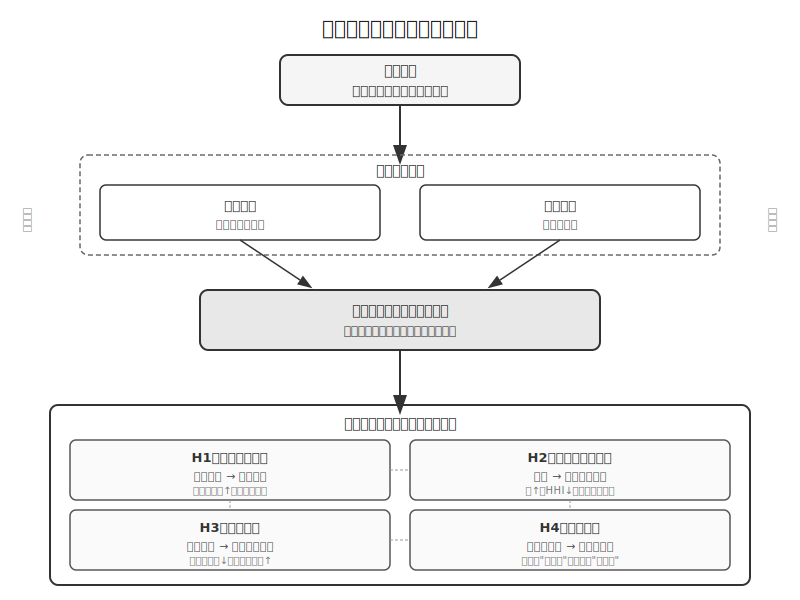
\includegraphics[width=0.95\textwidth]{figures/framework.png}
\caption{理论分析框架}
\label{fig:framework}
\end{figure}
